\section{Результати}

Отримані в ході експериментів числові показники точності (таб. \ref{tab:models-comparison})
та результуючі зображення дозволяють провести детальний порівняльний аналіз
алгоритмів за ступенем їх придатності до задачі перенесення колірного простору
між супутниковими знімками.

Для оцінки якості моделювання було використано шість стандартних метрик регресії:
коефіцієнт детермінації ($R^{2}$), частку поясненої дисперсії (\textit{Explained
Variance Score}), максимальну похибку (\textit{Max Error}), середню абсолютну
похибку (\textit{MAE}), середньоквадратичну похибку (\textit{MSE}) та медіанну абсолютну
похибку (\textit{Median AE}).

\begin{table}[H]
	\centering
	\caption{Порівняльна оцінка точності алгоритмів регресії та машинного навчання}
	\label{tab:models-comparison}
	\vspace{2mm}
	\small
	\begin{tabular}{|l|r|r|r|r|r|}
		\hline
		\textbf{Метрика точності} & \textbf{Лінійна}      & \textbf{Поліном.}     & \textbf{Баєсова}    & \textbf{Випадковий ліс} & \textbf{MLP}     \\
		\hline
		Explained variance        & $-2,26 \cdot 10^{23}$ & $-1,69 \cdot 10^{22}$ & $-0,18$             & 0,76                    & \textbf{0,81}    \\
		\hline
		Max error                 & $1,62 \cdot 10^{16}$  & $1,03 \cdot 10^{17}$  & 6532,00             & 4143,13                 & \textbf{3334,50} \\
		\hline
		Mean absolute error       & $2,52 \cdot 10^{14}$  & $5,36 \cdot 10^{11}$  & 638,81              & 385,0                   & \textbf{343,77}  \\
		\hline
		Mean squared error        & $2,02 \cdot 10^{29}$  & $1,51 \cdot 10^{28}$  & $1,31 \cdot 10^{6}$ & 368,11                  & \textbf{178,39}  \\
		\hline
		Median abs. error         & $1,22 \cdot 10^{14}$  & $2,35 \cdot 10^{6}$   & 183,60              & 102,20                  & \textbf{64,83}   \\
		\hline
		R2 score                  & $-2,26 \cdot 10^{23}$ & $-1,69 \cdot 10^{22}$ & $-0,46$             & 0,67                    & \textbf{0,72}    \\
		\hline
	\end{tabular}
\end{table}

\subsection{Лінійна та Поліноміальна регресії}

Первинне тестування базових математичних моделей виявило їхню повну
непридатність для розв'язання поставленої задачі (рис. \ref{fig:linear-and-polynomial-results}).

\begin{figure}[H]
  \centering
  \subfloat[Лінійна]{
    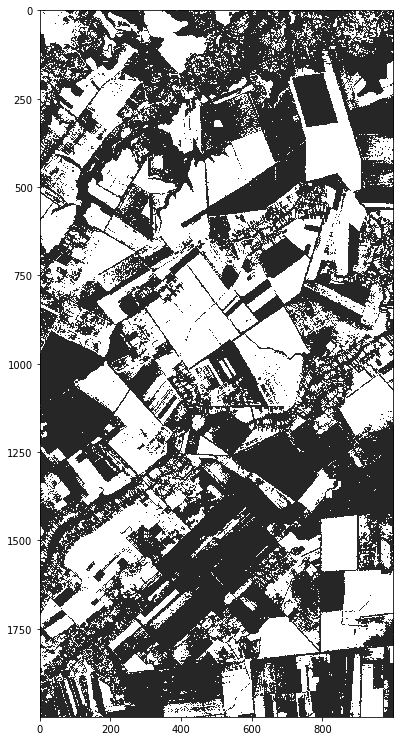
\includegraphics[width=0.4\textwidth]{images/image25}
  }
  \subfloat[Поліноміальна]{
    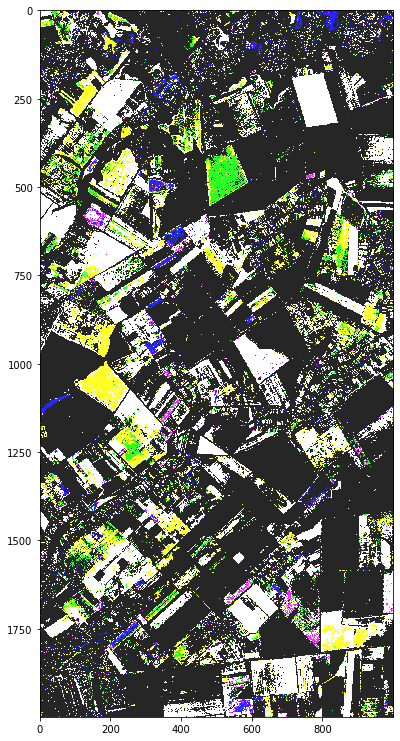
\includegraphics[width=0.4\textwidth]{images/image26}
  }
  \caption{Демонстрація роботи лінійної та поліноміальної регресій
    \label{fig:linear-and-polynomial-results}
  }
\end{figure}

\begin{itemize}
	\item \textbf{Лінійна регресія} показала критично незадовільні результати. Показники
		$R^{2}$ та \textit{Explained Variance} набули аномальних від'ємних значень
		порядку $-2,26 \cdot 10^{23}$, що свідчить про повну неадекватність моделі ---
		її передбачення виявилися значно гіршими, ніж банальне усереднення цільових
		значень. Середньоквадратична похибка ($\text{MSE}\approx 2,02 \cdot 10^{29}$)
		та середня абсолютна похибка ($\text{MAE}\approx 2,52 \cdot 10^{14}$) підтверджують
		наявність катастрофічних відхилень у спектральних каналах. Причиною цього є
		надмірна спрощеність лінійної моделі: залежність колірних спектрів супутникових
		знімків має складний нелінійний характер, який неможливо описати простим
		лінійним перетворенням.

	\item \textbf{Поліноміальна регресія} (з максимально можливим ступенем полінома
		$n=6$, обмеженим наявними обчислювальними ресурсами) продемонструвала деяке покращення
		порівняно з лінійною. Зорієнтовані метрики похибок знизилися на кілька
		порядків (наприклад, $\text{MAE}$ впала до $5,36 \cdot 10^{11}$, а $\text{MSE}$
		--- до $1,51 \cdot 10^{28}$). Проте коефіцієнт детермінації ($R^{2}\approx -
		1,69 \cdot 10^{22}$) залишається глибоко у від'ємній зоні, а максимальна
		похибка ($\text{Max Error}\approx 1,03 \cdot 10^{17}$) навіть зросла
		порівняно з лінійним наближенням. Це пояснюється явищем прокляття розмірності
		та явищем перенавчання (оверфітингу) поліномів високого степеня на межах діапазонів
		значень пікселів. Візуально знімки після такої обробки містять суттєві
		спотворення кольорів та артефакти.
\end{itemize}

\subsection{Баєсова регресія}

Застосування \textbf{баєсової регресії} стало першим кроком до виходу із зони екстремально
великих похибок (рис. \ref{fig:bayesian-result}). Впровадження регуляризації та
апріорного розподілу параметрів дозволило стабілізувати процес навчання та уникнути вибуху градієнтів/ваг.

\begin{figure}[H]
  \centering
  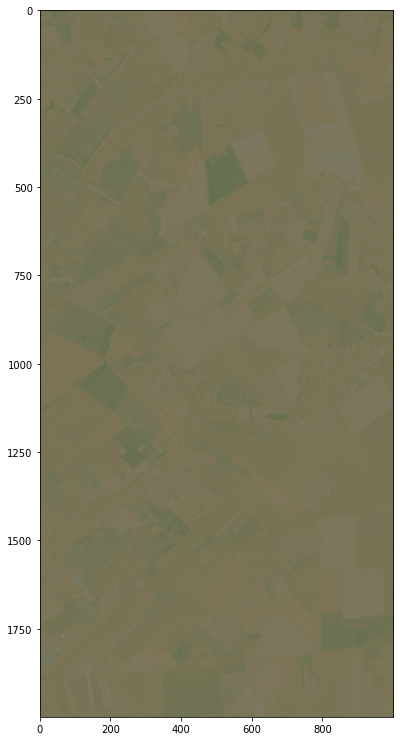
\includegraphics[width=0.4\textwidth]{images/image27}
  \caption{Демонстрація роботи баєсової регресії}
  \label{fig:bayesian-result}
\end{figure}

Середня абсолютна похибка знизилася до прийнятного рівня у $638,81$ умовних
одиниць інтенсивності, а медіанна похибка ($\text{Median AE}$) склала $183,60$.
Значення $R^{2}$ ($-0,46$) та \textit{Explained Variance} ($-0,18$), хоч і
залишаються від'ємними, демонструють фундаментальний стрибок у якості порівняно з
попередніми методами. Модель змогла згладити глобальні колірні зсуви, однак візуальний
аналіз знімка свідчить про те, що локальні спектральні особливості та дрібні
деталі зображення передаються некоректно. Баєсова регресія виявилася недостатньо
гнучкою для адаптації до складних розподілів яскравості на неоднорідних ділянках
(наприклад, межа «вода--рослинність»).

\subsection{Ансамблеві та нейромережеві підходи}

Справжній якісний прорив у точності синтезу колірного простору було досягнуто
лише за допомогою алгоритмів машинного та глибокого навчання (рис. \ref{fig:random-forest-mlp}).

\begin{figure}[H]
  \centering
  \subfloat[Випадковий ліс]{
    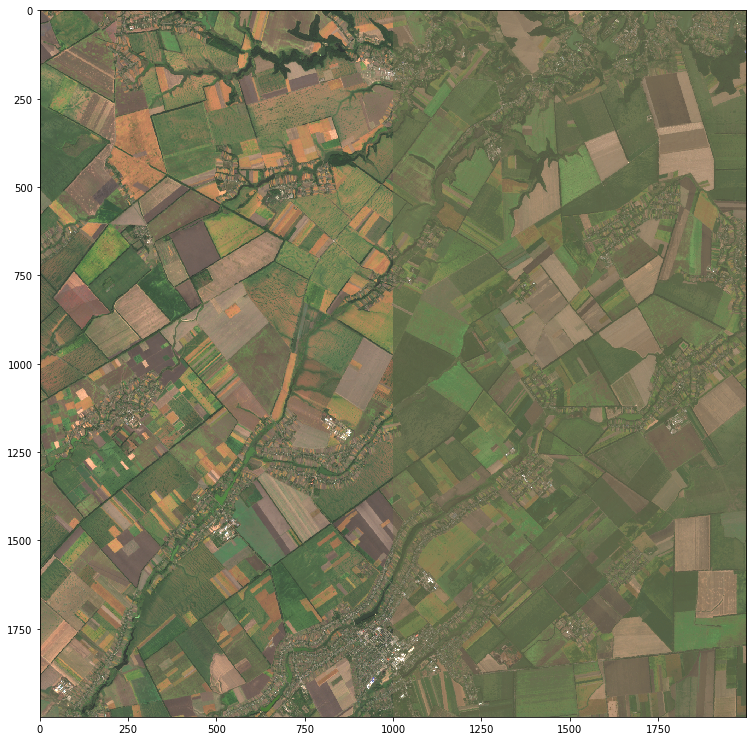
\includegraphics[width=0.45\textwidth]{images/image28}
  }
  \subfloat[Багатошаровий перцептрон]{
    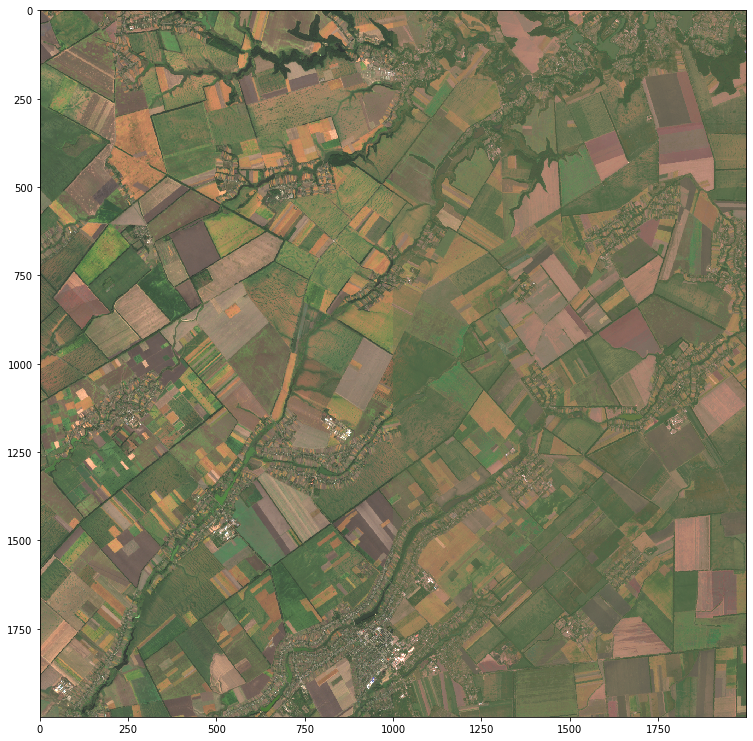
\includegraphics[width=0.45\textwidth]{images/image29}
  }
  \caption{Демонстрація роботи випадкового лісу та багатошарового перцептрона
    \label{fig:random-forest-mlp}
  }
\end{figure}

\begin{itemize}
	\item \textbf{Випадковий ліс (Random Forest):} Цей ансамблевий алгоритм
		показав високу ефективність у моделюванні складних нелінійних залежностей. Показник
		$R^{2}$ досяг $0,67$, а частка поясненої дисперсії — $0,76$. Середня абсолютна
		похибка ($\text{MAE}$) знизилася орієнтовно до $385,00$, а
		середньоквадратична похибка ($\text{MSE}$) склала $368,11$. Медіанна похибка
		скоротилася майже вдвічі порівняно з Баєсовою регресією (до $102,20$).

	\item \textbf{Багатошаровий перцептрон (MLP):} Нейромережева модель показала
		\textbf{найкращий результат} серед усіх досліджуваних методик за кожною без винятку
		метрикою:
		\begin{itemize}
			\item $R^{2}= 0,72$ та \textit{Explained Variance} $= 0,81$, що свідчить про
				високу здатність моделі пояснювати варіативність колірного простору цільового
				знімка.

			\item $\text{MAE}= 343,77$ (майже вдвічі менше, ніж у Баєсової регресії та
				Випадкового лісу).

			\item $\text{MSE}= 178,39$ (найнижче значення серед усіх моделей, що підтверджує
				відсутність грубих викидів).

			\item $\text{Median AE}= 64,83$, що вказує на те, що для переважної більшості
				пікселів похибка перенесення кольору є мінімальною та непомітною для людського
				ока.

			\item $\text{Max Error}= 3334,50$ (мінімальна максимальна похибка серед
				усіх методів).
		\end{itemize}
\end{itemize}
